The domain is a unit cube. Free slip boundary conditions 
are imposed on all sides. The mesh counts 
nelx*nely*nelz=nel elements and 
nnx*nny*nnz=NV nodes.
The density and the viscosity are prescribed in the domain 
by means of two functions:
the density is set to 2 inside a sphere of radius 0.123 centered 
at (0.5,0.5,0.5) and 1 outside. The viscosity is 100 inside the sphere
and 1 outside.  The gravity vector is set to $\vec{g}=(0,0,-1)$.

The FE matrix size grows even faster now than in the previous 2D case so
choosing the right matrix storage is of paramount importance. 

Three experiments are carried out:
\begin{enumerate}
\item the one described above.
We see that the pressure field is dominated by the lithostatic signal.
\item same as experiment 1, but a reference density of 1 is substracted to all densities, so that 
the sphere density is 1 and the density of the surrounding fluid is now 0. In essence, we remove a
'background' density which does not participate in the flow generation, and thereby get rid of the 
lithostatic signal of the pressure.
\item same as experiment 2, but the top boundary is now open (free surface)
\end{enumerate} 


\begin{center}
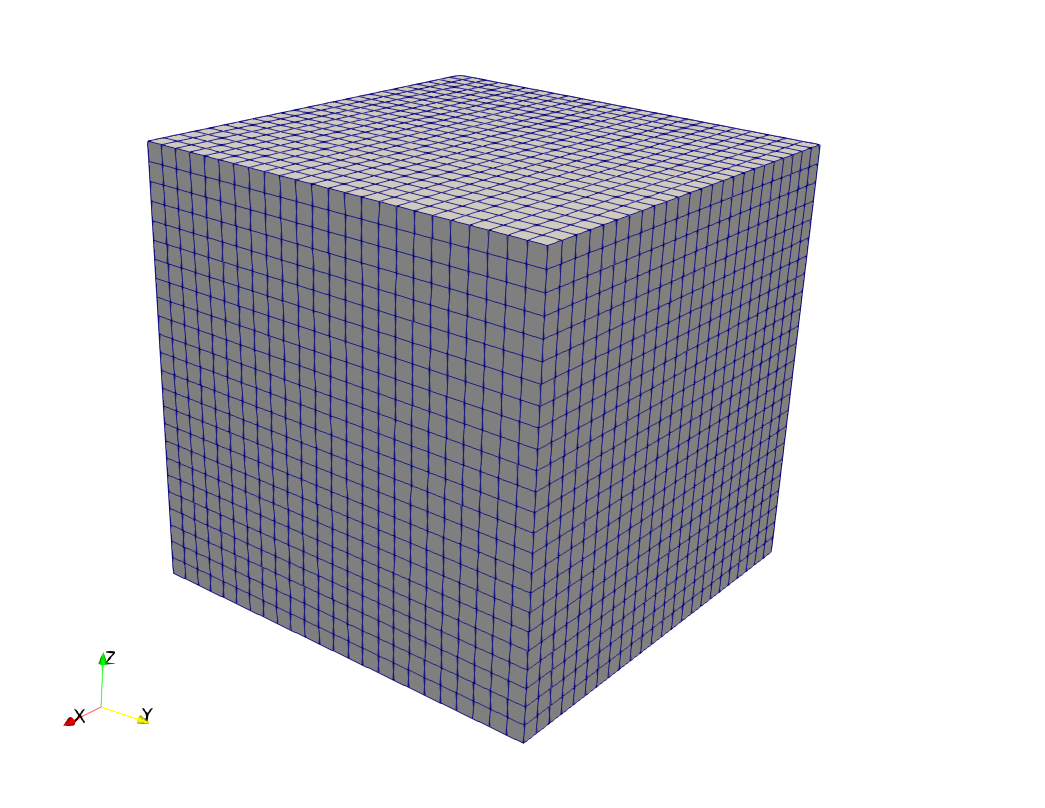
\includegraphics[width=5cm]{python_codes/fieldstone_10/results/grid}
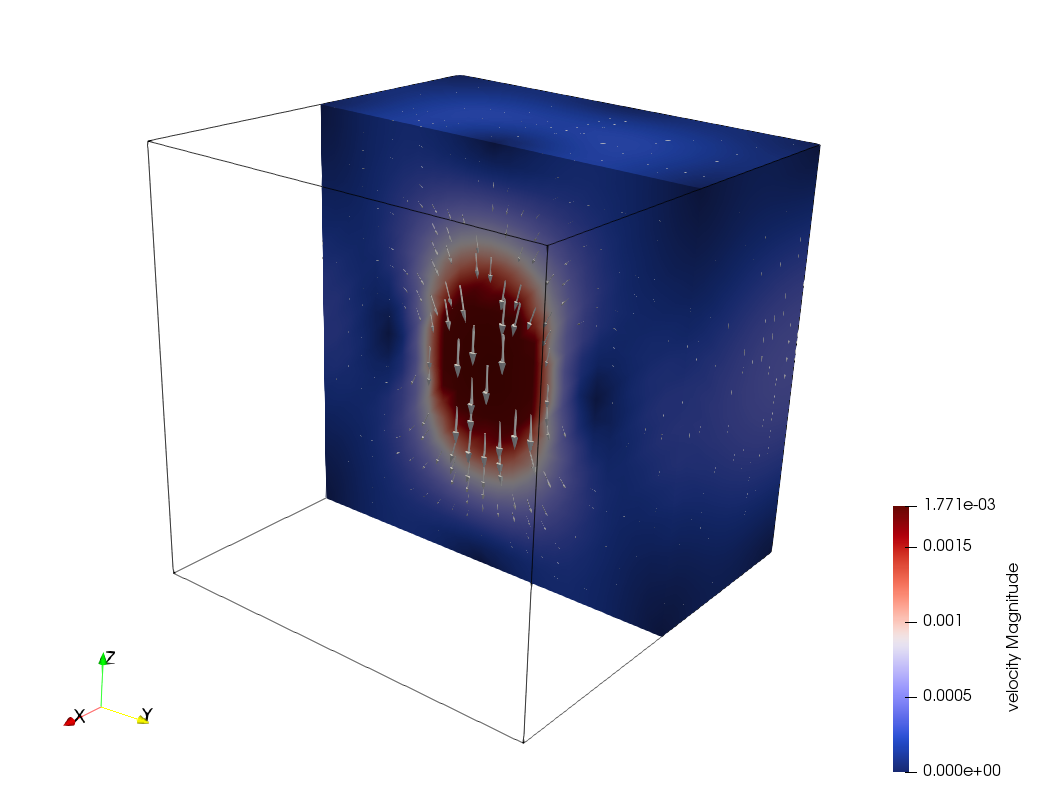
\includegraphics[width=5cm]{python_codes/fieldstone_10/results/vel}
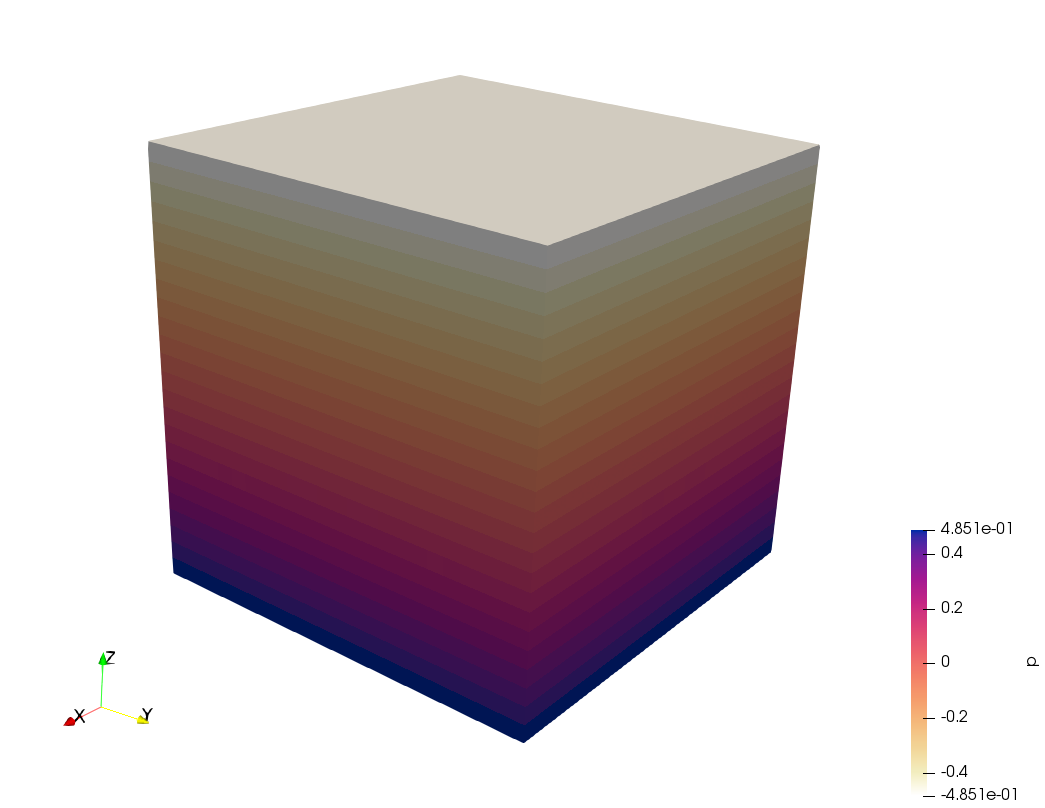
\includegraphics[width=5cm]{python_codes/fieldstone_10/results/press}\\
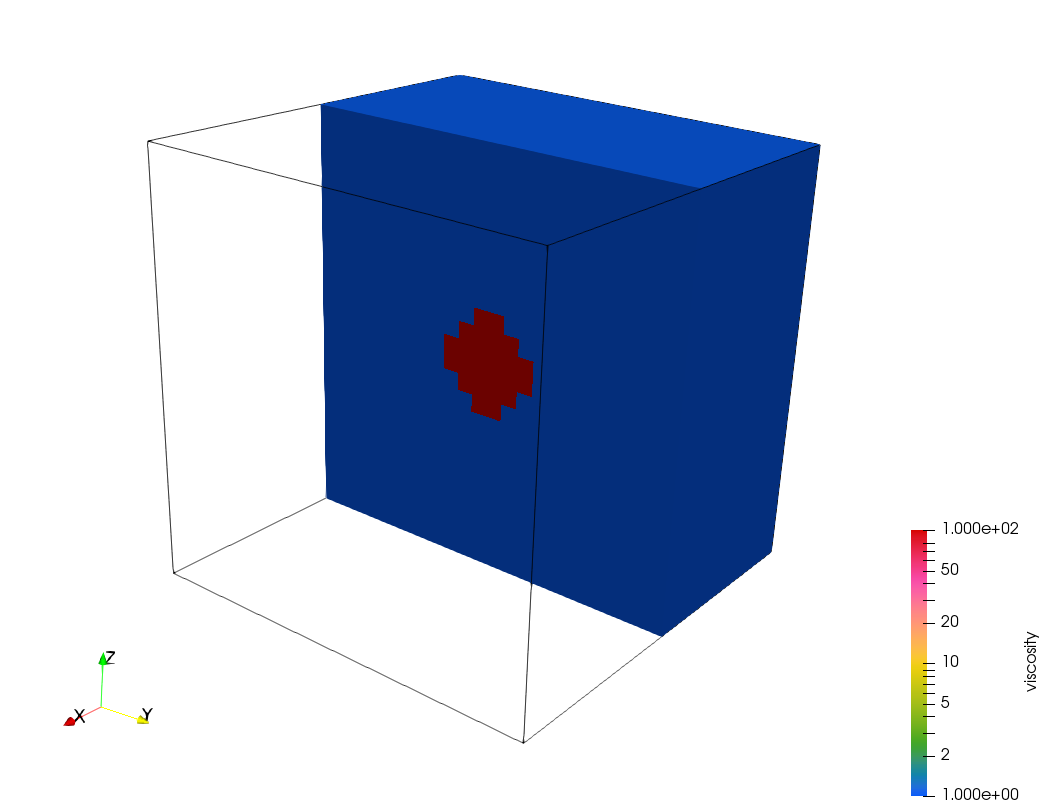
\includegraphics[width=5cm]{python_codes/fieldstone_10/results/visc}
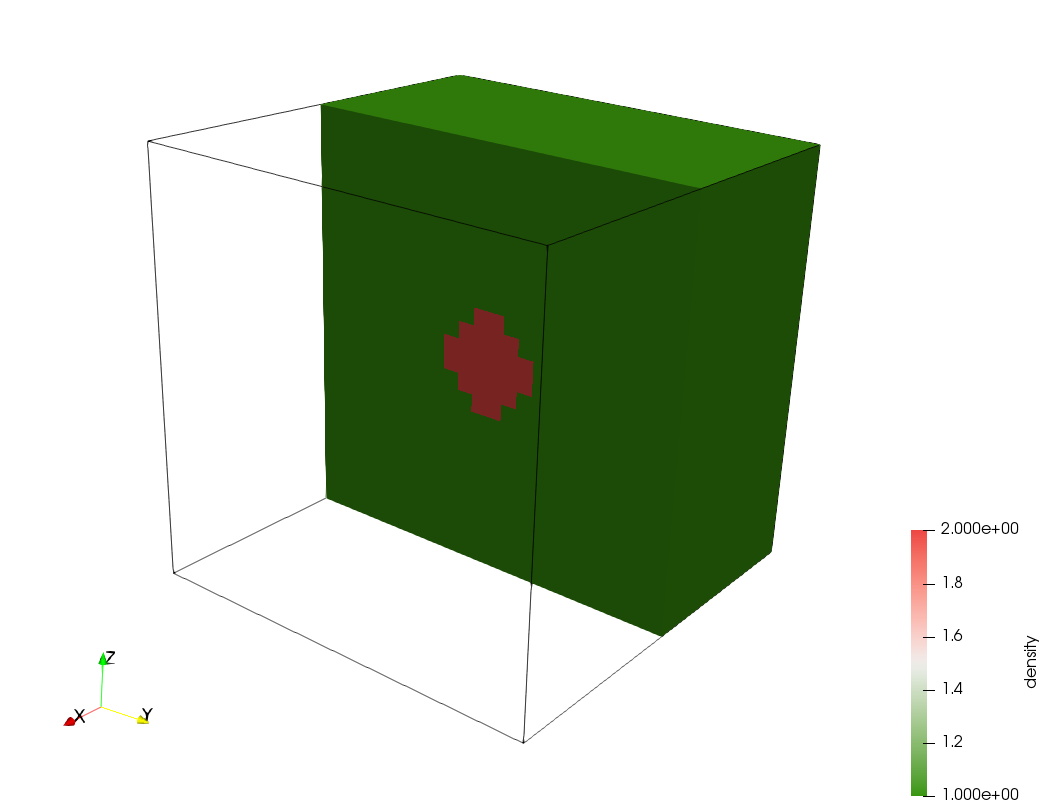
\includegraphics[width=5cm]{python_codes/fieldstone_10/results/dens}\\
{\small Experiment 1: resolution 24x24x24}
\end{center}

\begin{center}
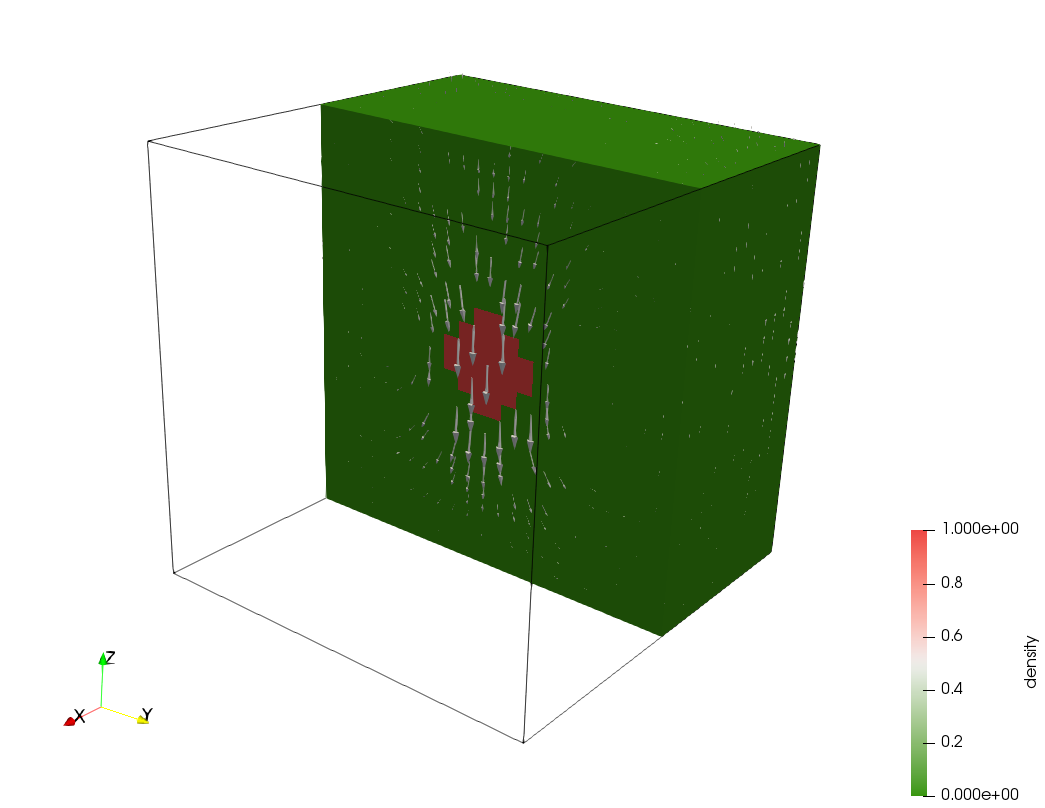
\includegraphics[width=5cm]{python_codes/fieldstone_10/results/dens_2}
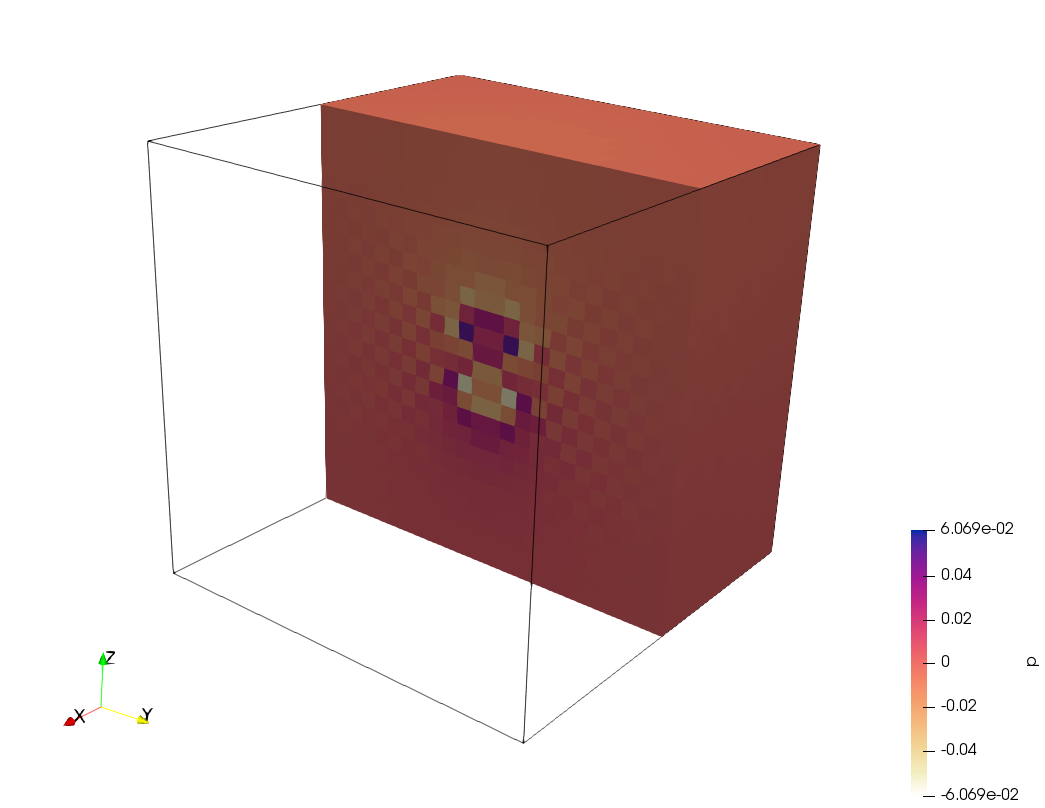
\includegraphics[width=5cm]{python_codes/fieldstone_10/results/press_2}\\
{\small Experiment 2: Density and pressure fields. Resolution 24x24x24}
\end{center}


\begin{center}
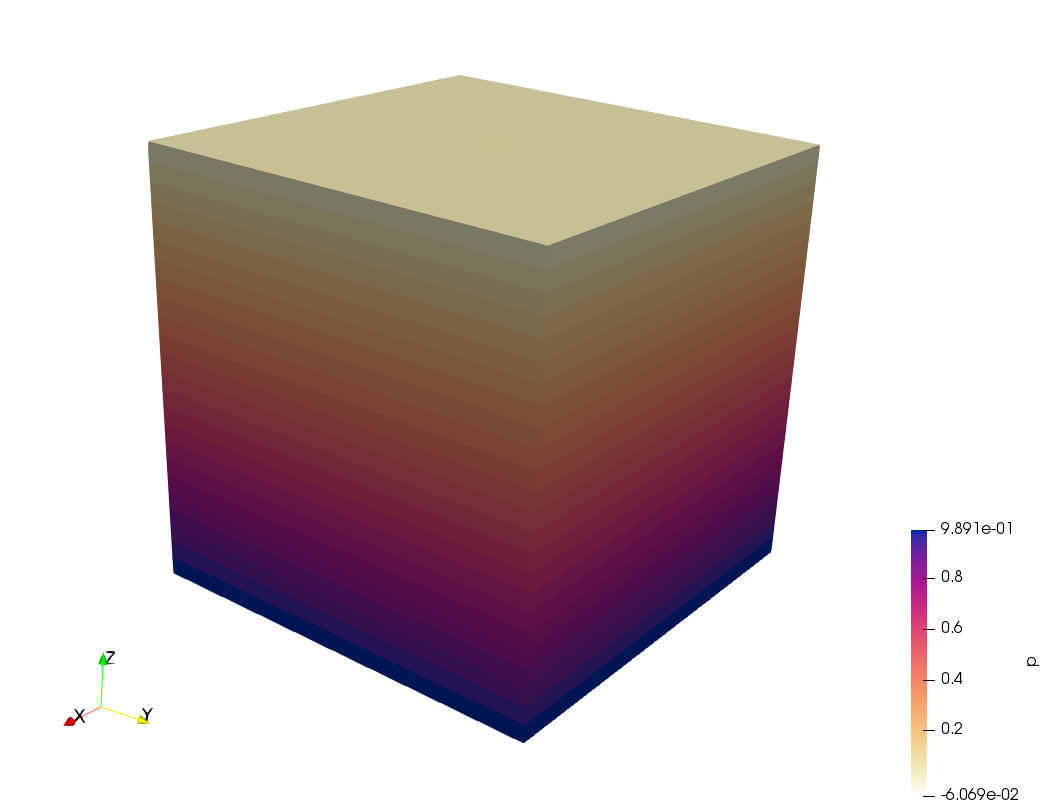
\includegraphics[width=5cm]{python_codes/fieldstone_10/results/press_3}
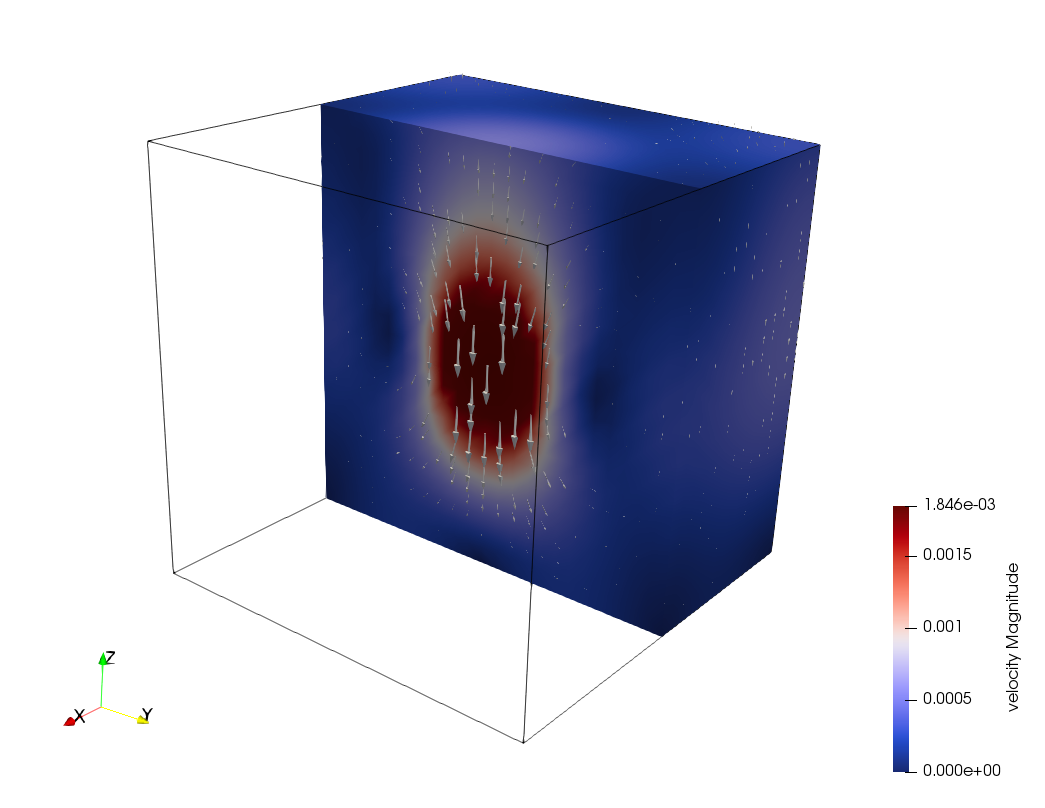
\includegraphics[width=5cm]{python_codes/fieldstone_10/results/vel_3}\\
{\small Experiment 3: pressure and velocity fields. Resolution 24x24x24}
\end{center}




\begin{center}
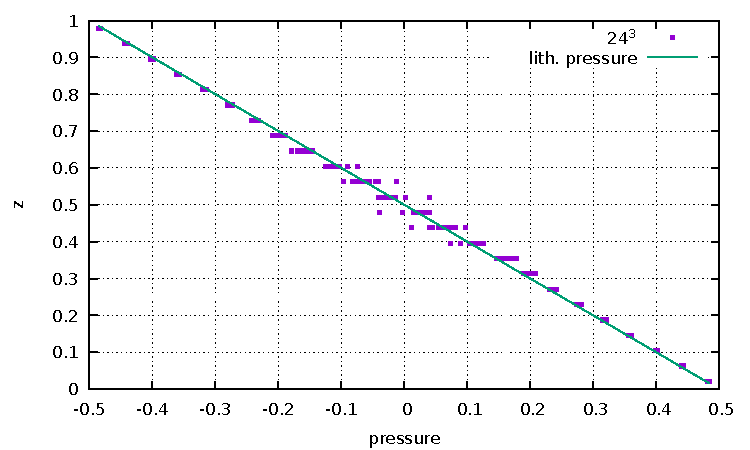
\includegraphics[width=5cm]{python_codes/fieldstone_10/results/model1/pressure.pdf}
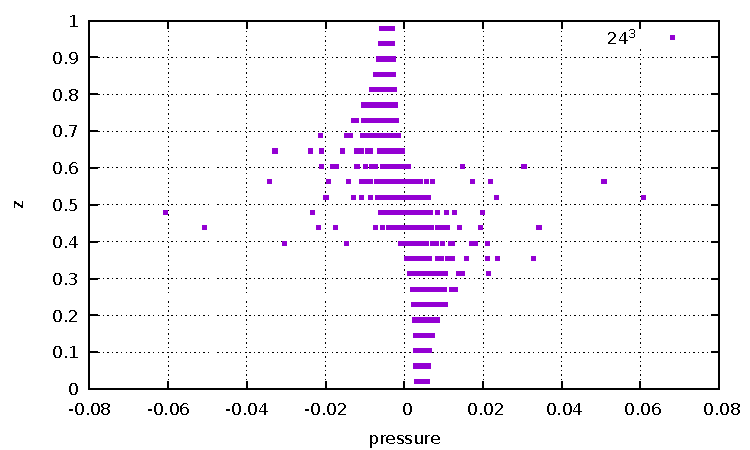
\includegraphics[width=5cm]{python_codes/fieldstone_10/results/model2/pressure.pdf}
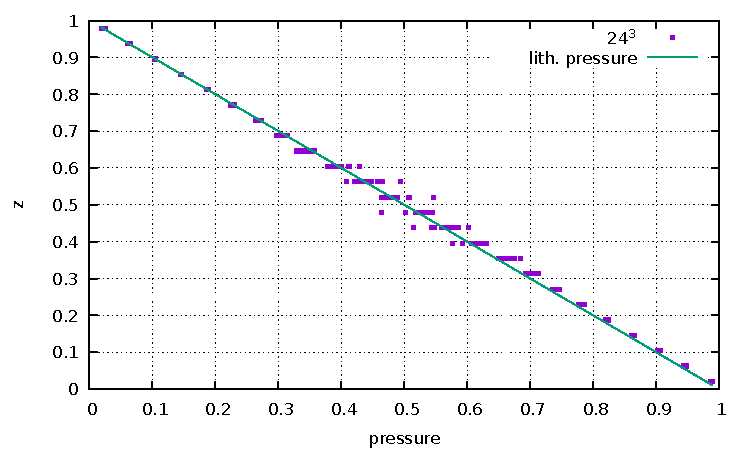
\includegraphics[width=5cm]{python_codes/fieldstone_10/results/model3/pressure.pdf}\\
{\captionfont Elemental pressure for all elements as a function of their vertical (middle) coordinate for
(from left to right) experiments 1, 2 and 3. }
\end{center}
